\documentclass[aspectratio=169]{beamer}
\usepackage{tikz}
\usetikzlibrary{shadows}
\usepackage{listings}
\usepackage[natbibapa]{apacite}
\makeatletter
\NAT@longnamesfalse
\makeatother

\beamertemplatenavigationsymbolsempty
\setbeamercolor{bluebox}{bg=blue!10}
\newenvironment{colbox}[1][\textwidth]%
  {\begin{beamercolorbox}[wd=#1, rounded=true, shadow=true]{bluebox}}
  {\end{beamercolorbox}}
\setbeamertemplate{footline}{\vskip-6pt\hfill\insertframenumber$\;$\vskip1pt}

\lstdefinestyle{numbers}{language=R,%
  basicstyle=\ttfamily\small\color{blue!50!black},%
  commentstyle=\slshape\color{gray!40!black},%
  numbers=left,numberstyle=\tiny\color{gray!40!black},%
  basewidth={.5em, .4em},%
  showstringspaces=false}

\lstset{language=R,%
  basicstyle=\ttfamily\small\color{blue!50!black},%
%  frame=single,%
  commentstyle=\slshape\color{gray!40!black},%
%  keywordstyle=\bfseries\color{blue!50!black},%
%  identifierstyle=\color{blue!50!black},%
%  stringstyle=\color{green!40!black},%
%  numbers=left,numberstyle=\tiny,%
  upquote=true,%  straight single quotes for python
  basewidth={.5em, .4em},%
  showstringspaces=false,%
  emphstyle=\color{red}}


\begin{document}

\title{Power Analysis \&\\
       Sample Size Calculation\\[2ex]

\small (Require Substance-Matter Knowledge)}

\author{}
\date{Last modified: 2025-04-13}

\begin{frame}
\thispagestyle{empty}
\titlepage
\end{frame}

% Welcome everybody, let me introduce myself

% Goal: nobody leaves without having done their own power analysis
% Technical problem: easy
% Substantive problem: difficult
%
% We wanna infer sth about the real world, we're gonna have to invite
%  the real world in


\begin{frame}{Overview}

\begin{itemize}
\item Large effects from subtle manipulations?
\item Inference and power
\item Power analysis by simulation
\item Do it yourself
\end{itemize}

\end{frame}

% Here is my overview: I want to introduce with some examples what we get if
% we don't care about power; then introduce power and power simulation; and
% then do some hands-on exercises with you.


%%%%%%%%%%%%%%%%%%%%%%%%%%%%%%%%%%%%%%%%%%%%%%%%%%%%%%%%%%%%%%%%%%%%%%%%%%%%%
\section{Large effects from subtle manipulations?}
%%%%%%%%%%%%%%%%%%%%%%%%%%%%%%%%%%%%%%%%%%%%%%%%%%%%%%%%%%%%%%%%%%%%%%%%%%%%%


\begin{frame}{Help, my effect size is too large!}

Examples
\begin{itemize}
\item Decision biases from two-hand tapping
\item Beautiful parents have more daughters
\end{itemize}

\end{frame}

% Probably never heard anyone complain about this;
% but it's a huge problem for the scientific integrity of our field:
% Reported effect sizes are way too large.
%
% Before explaining the reasons for this, let's have a look at two examples:
% Decision ... and the notorious beautiful parents.


\begin{frame}{Refresher: Framing}

\begin{itemize}
\item \citet{ TverskyKahneman81}\\[1ex]

``Imagine that the U.S.\ is preparing for the outbreak of an unusual Asian
disease, which is expected to kill 600 people. Two alternative programs to
combat the disease have been proposed'' (p.~453)\\[1ex]

\begin{columns}
\begin{column}{0.4 cm}
\end{column}
%
\begin{column}{5.8 cm}
\begin{colbox}
If Program A is adopted \textbf{200} people will be \textbf{saved} [109]\\[2ex]

If Program B is adopted there is 1/3 probability that \textbf{600} people
will be \textbf{saved}, and 2/3 probability that \textbf{no people} will be
\textbf{saved} [43]
\end{colbox}
\end{column}
%
\begin{column}{5.8 cm}
\begin{colbox}
If Program C is adopted \textbf{400} people will
\textbf{die} [34]\\[2ex]

If Program D is adopted there is 1/3 probability that \textbf{nobody} will
\textbf{die}, and 2/3 probability that\\
\textbf{600} people will \textbf{die} [121]
\end{colbox}
\end{column}
\end{columns}

\vspace{2ex}

\item Odds ratio (OR) $=$ 9.0
\end{itemize}
\end{frame}

% In their classic study of the framing effect, TverskyKahneman81 presented a
% decision dilemma about a new disease. Participants have to decide between
% two options, a safe and a risky option. And, there are two versions of the
% dilemma: In the gain version, you can either gain a certain number of lives
% for sure or you gain everyone's lives with a certain probability (or no
% one's). In the loss version, you loose a number of lives or have the chance
% to loose no one (or everybody). It turned out that participants avoid taking
% the risk under gain framing, but not under loss framing; an indication of
% irrational behavior.


\begin{frame}[fragile]{Decision biases from two-hand tapping}

\begin{itemize}
\item \citet{McElroySeta04}, $n = 48$\\[1ex]

``a behavioral task of finger tapping was used to induce asymmetrical
activation of the respective hemispheres \dots Framing effects were found when
the right hemisphere was selectively activated whereas they were not observed
when the left hemisphere was selectively activated'' (p.~572)

\begin{lstlisting}
     right-hand tapping  left-hand tapping  ratio of odds
     safe risky          safe risky         ratios (ROR)
gain    8     4            12     1
loss    7     4             3     9
OR          1.1                  36         31.5
\end{lstlisting}

\item Our replication \citep[see][]{Gelman20}, $n = 332$
\begin{lstlisting}
gain   52    31            56    27
loss   26    57            30    53
OR          3.7                 3.7          1.0
\end{lstlisting}
\end{itemize}

\end{frame}

% Now, McElroySeta04 wanted to manipulate the framing effect. Here's what they
% did.

% What I want to illustrate here is that given such a subtle manipulation the
% effect is huge. Here is another well-known example.


\begin{frame}{Beautiful parents have more daughters}

\begin{columns}
\begin{column}{5.6cm}
\begin{itemize}
\item \citet{Kanazawa07}\\[1ex]

``Very attractive individuals are 26\% less likely to have a son''
(p.~133)\\[1ex]

-- $n_{total} = 2970$\\
-- $n_{v.att.} < 400$\\[2ex] % "11.2% are so rated by the interviewer" (p. 136)

\item \citet{GelmanWeakliem09}\\[1ex]

``the noise is stronger than the signal'' (p.~314)
\end{itemize}
\end{column}
%
\begin{column}{8.6cm}
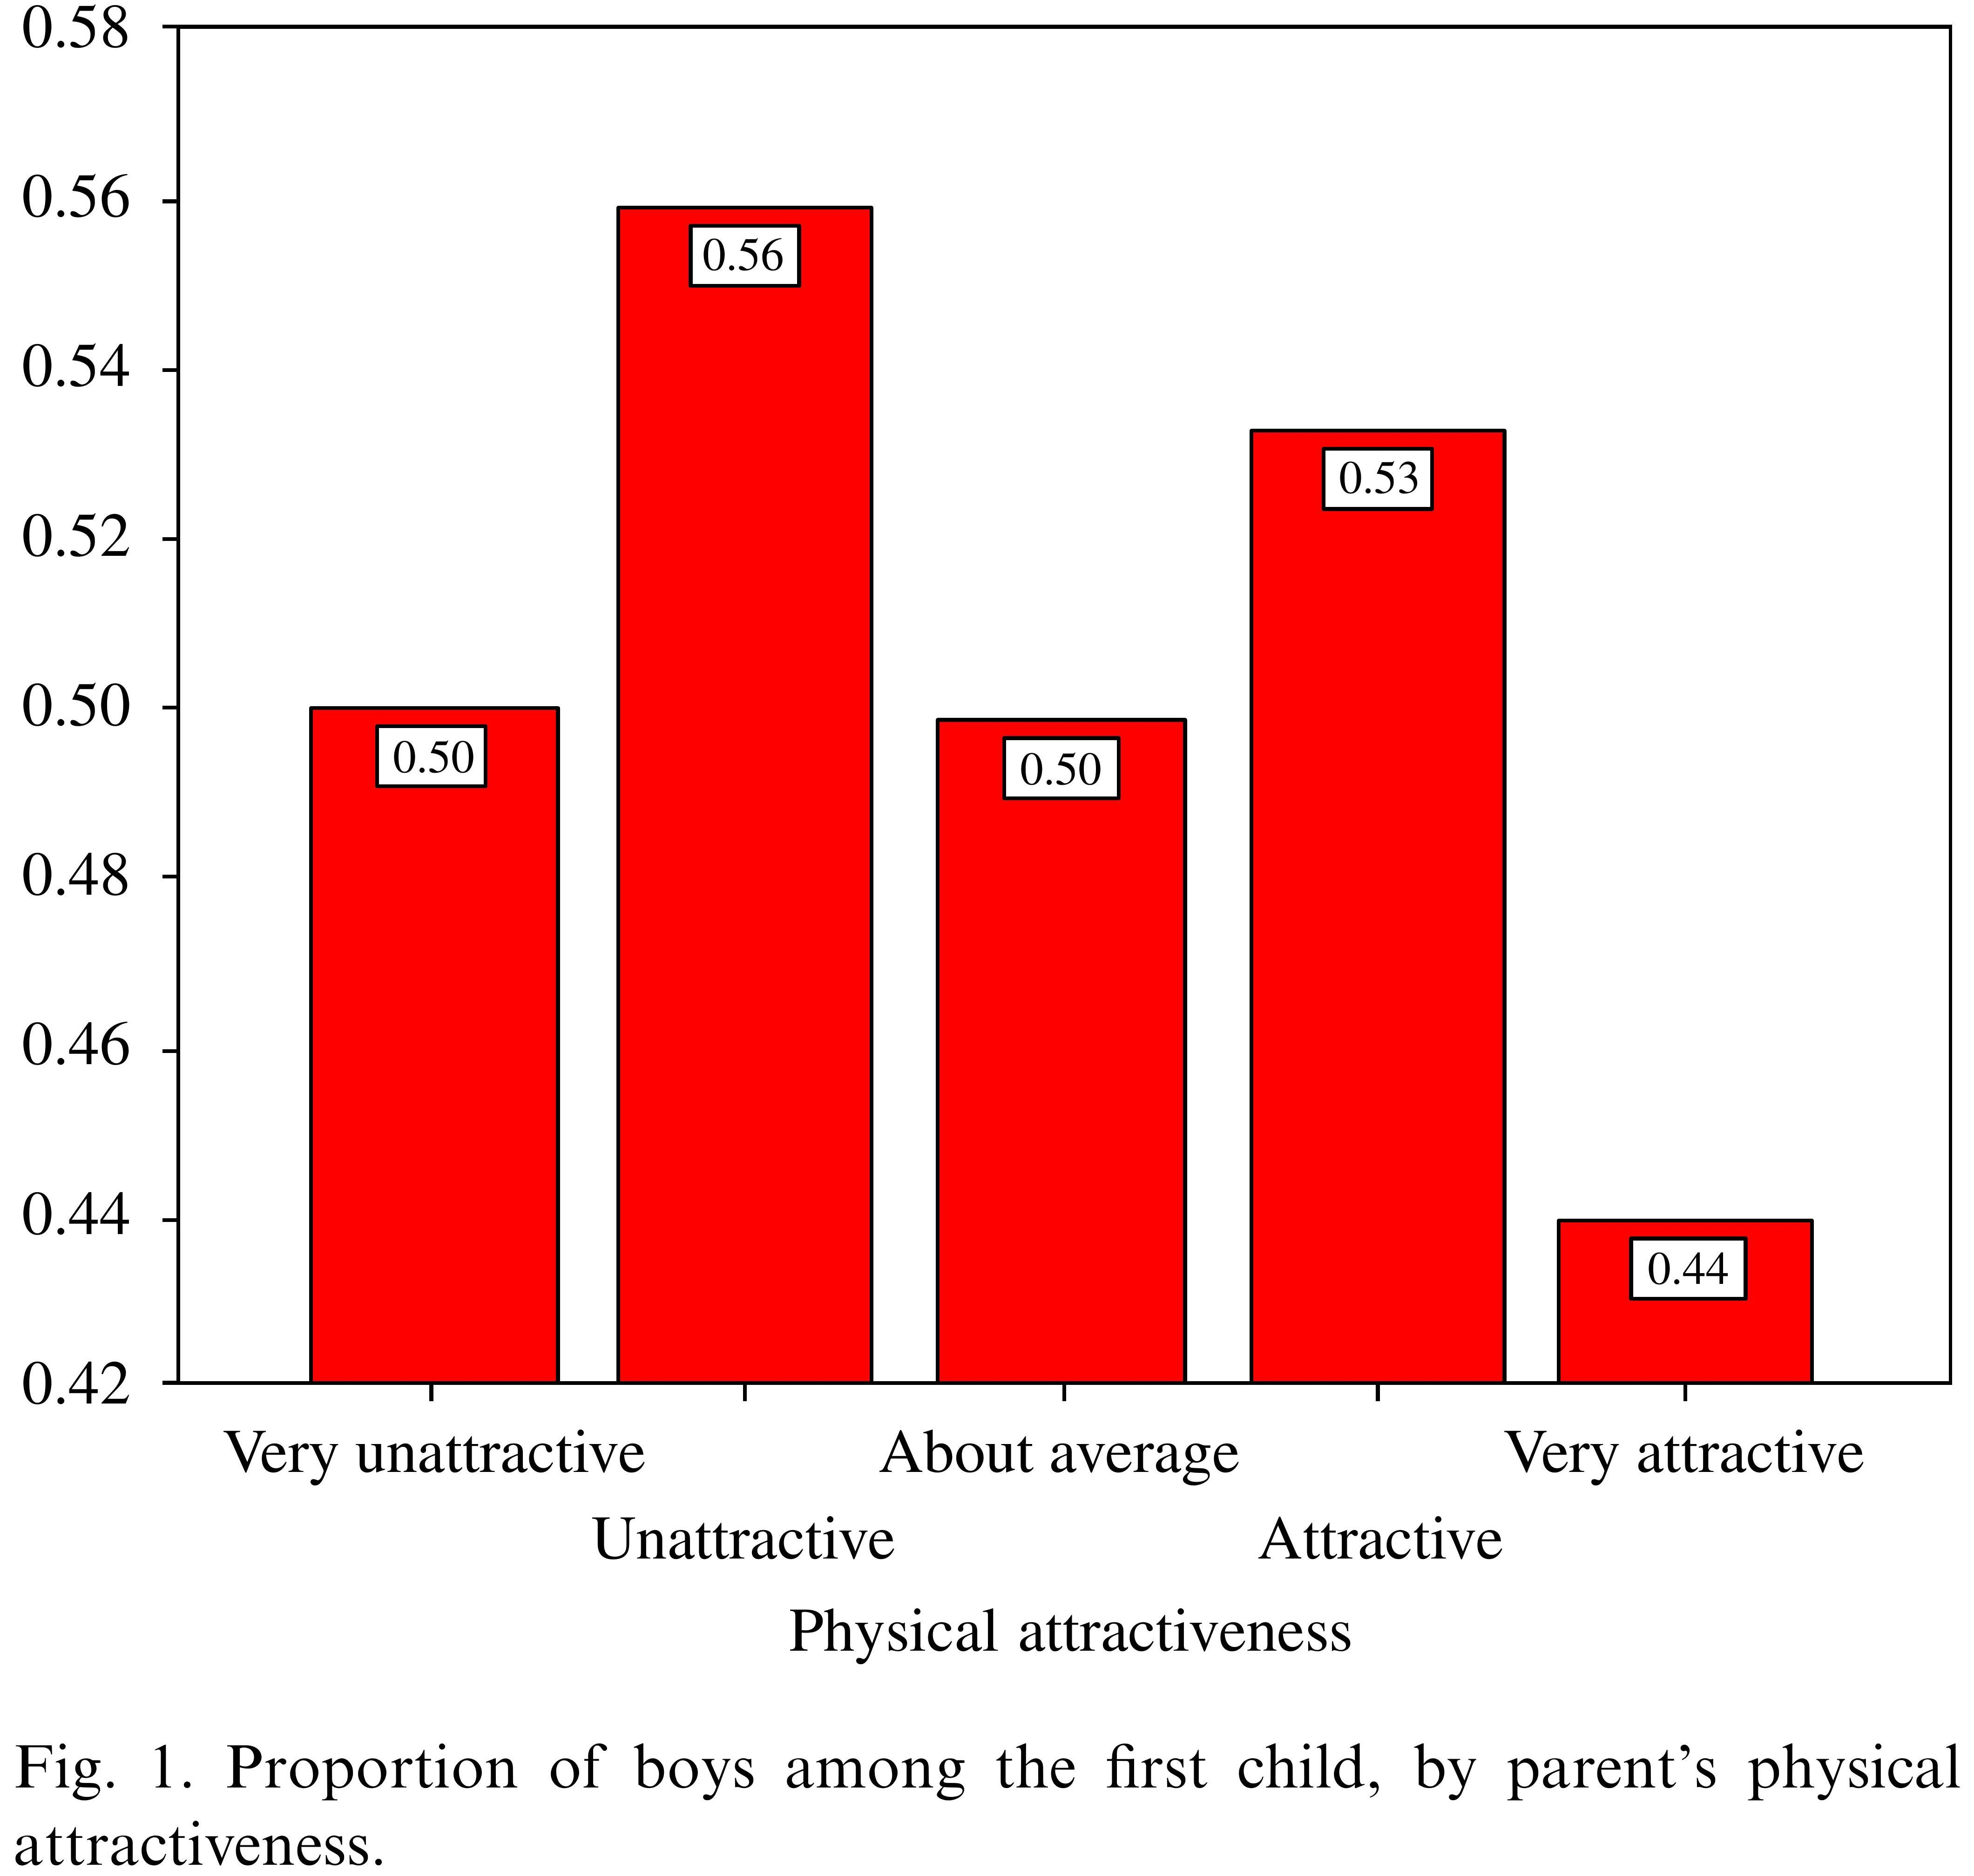
\includegraphics[width=8.5cm]{fig/Kanazawa}
\end{column}
\end{columns}

\end{frame}

% In the normal population, there are about 51.5% (or 106:100) boy births. But
% Kanazawa07 found that ...

% exp(coef(glm(cbind(c(1371, 147), c(1265, 186)) ~ I(0:1), binomial)))
% OR ~= .74 -> "26% less likely"

% This is a biologically implausible effect, way too large.

% GelmanWeakliem09: Our reaction when seeing such large estimates was not
% "Wow, they've found something big!" but, rather, "Wow, this study is under
% powered!"


\begin{frame}{Large effects from subtle manipulations?}

There is a simple explanation for the seemingly large effects published all
over the psychological literature\\[2ex]

\begin{itemize}
\item that works without any real large effects

\item but assumes that they are statistical artifacts based on a combination
of\\[2ex]

~\hfill\begin{colbox}[5cm]
\centering
low power\\
$\wedge$\\
selection by significance\\[1ex]
\hrule\vspace{1ex}
$\Rightarrow$ inflated effect
\end{colbox}\hfill~

\vspace{2ex}

\citep[type M error;][]{GelmanCarlin14}
\end{itemize}

\end{frame}

% So, what's going on with these large effects from subtle manipulations?
% Are we really surrounded by these large effects?
% I'd say no, there is a simpler explanation.
%
% or: winner's curse, statistical significance filter
%
% What I am saying here is \emph{not} that it {\bf may} happen that effects
% will be inflated but that it {\bf must} happen

% In such a setting, effect size is a function of the sample size:
%   small samples => spectacular effects
% Don't make your effects a function of the sample size!
%
% In order to understand the mechanism behind this, let's have a short recap
% of statistical inference.


%%%%%%%%%%%%%%%%%%%%%%%%%%%%%%%%%%%%%%%%%%%%%%%%%%%%%%%%%%%%%%%%%%%%%%%%%%%%%
\section{Inference and power}
%%%%%%%%%%%%%%%%%%%%%%%%%%%%%%%%%%%%%%%%%%%%%%%%%%%%%%%%%%%%%%%%%%%%%%%%%%%%%


\begin{frame}{Classical inference in a nutshell}

\begin{itemize}
\item Deciding between two hypotheses about parameter of data-generating
model \citep{NeymanPearson33}

\item Null hypothesis (specific), alternative hypothesis (logical opposite)\\
-- Example: Binomial model, H$_0$: $\pi = 0.5$, H$_1$: $\pi \neq 0.5$

\item Possible decision errors\\[1ex]

\renewcommand{\arraystretch}{1.2}
\begin{columns}
\begin{column}{7cm}
\begin{colbox}[7.6cm]
\centering
\begin{tabular}{l|c|c|}
\multicolumn{1}{l}{} & \multicolumn{1}{c}{Decision for H$_0$}
 & \multicolumn{1}{c}{Decision for H$_1$}\\ \cline{2-3}
H$_0$ true & correct                & type I error, $\alpha$\\ \cline{2-3}
H$_1$ true & type II error, $\beta$ & correct               \\ \cline{2-3}
\end{tabular}
\end{colbox}
\end{column}
%
\begin{column}{3cm}
Conventions
\begin{itemize}
\item $\alpha = 0.05$
\item $\beta < 0.2$
\end{itemize}
\end{column}
\end{columns}

\vspace{1ex}

\item Decision based on data (p-value)\\
-- If $p < \alpha$, choose H$_1$; else retain H$_0$

\item Power $= 1 - \beta$\\
-- Probability of test to detect an effect of a given size
\end{itemize}

\end{frame}

% In classical inference, a statistical test is a decision problem.

% As the parameter is unknown, we don't know which hypothesis is true. And we
% can be lucky with our decision or make one of two errors.

% In order to decide between H$_0$ and H$_1$, data will be collected and the
% test statistic and its p-value calculated. The p-value is the probability of
% obtaining a test statistic that signals a deviation from H$_0$ at least as
% extreme as that observed in the experiment, given H$_0$ is true and its
% underlying model holds. The decision rule is that if a test is significant
% so that its p-value is smaller than $\alpha$, then H$_1$ is chosen, else
% H$_0$ is retained.
% 
% An experiment should be designed so that it has a good chance to detect an
% interesting deviation from H$_0$. Such a deviation is called the effect
% size. The sample size of the experiment, $\alpha$, $\beta$, and the effect
% size are related. Fixing three of them allows one to determine the forth one
% \citep{Cohen92}. Power (also called true positive rate, hit rate,
% sensitivity, or recall) is defined as $1 - \beta$. It is the probability of
% a statistical test to detect an effect of a given size. Therefore, designing
% an experiment to have a good chance to find an effect means making sure its
% power is high enough.
%
% Power = prob of test to produce p < alpha; what affects this probability of
% a test to become significant?


\begin{frame}{Power function}

\begin{columns}
\begin{column}{4.5cm}
Power of a test depends on\\[1ex]

\begin{itemize}
\item effect size\\
(deviation from H$_0$)

\item sample size $n$

\item $\alpha$\\[2ex]
\end{itemize}

With effect size, power, and $\alpha$ fixed, we can calculate $n$
\end{column}
%
\begin{column}{10cm}
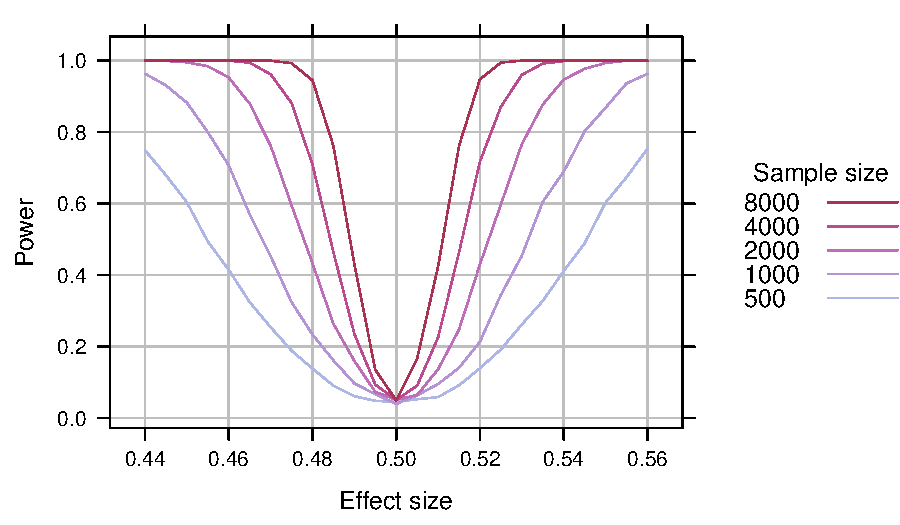
\includegraphics[width=10cm]{fig/OCbinomtest}
\end{column}
\end{columns}

\end{frame}

% - H0, H1, alpha, beta, power
% 
% - Power function of a test
%   o effect size, n, alpha, SD, power influence each other
% 
% - Type-M error and the statistical significance filter
%
% Can you spot alpha in the figure?
% The data model can produce output so outlandish that it seems incompatible
%   with H0; this will happen 5% of the time.
%
% Because of the functional dependency, if we fix effect size, n, and alpha,
%   we can calculate n; this is what we're gonna do in a minute.
%
% But first, let's understand why high power is so important; or: how low
% power destroys our inference.


\begin{frame}{High power is a necessary condition for valid inference}

\begin{columns}
\begin{column}{7.9cm}
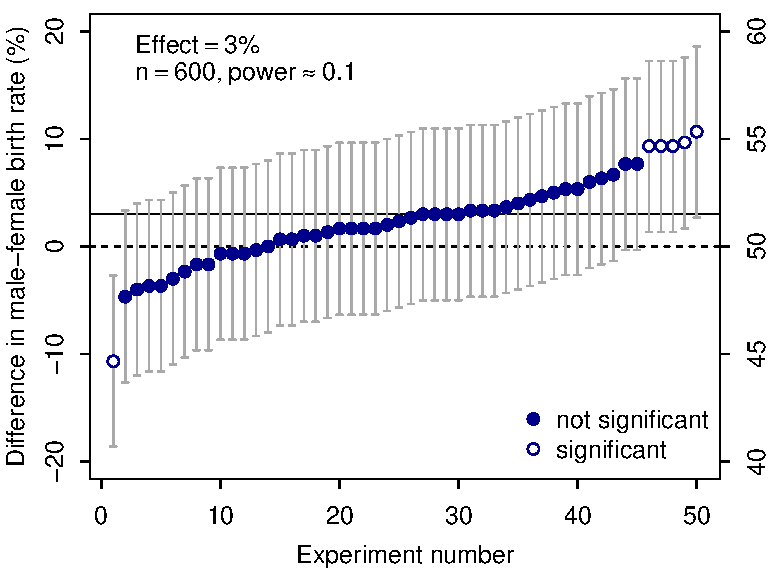
\includegraphics[width=7.9cm]{fig/birthdiff10}
\end{column}
%
\begin{column}{7.9cm}
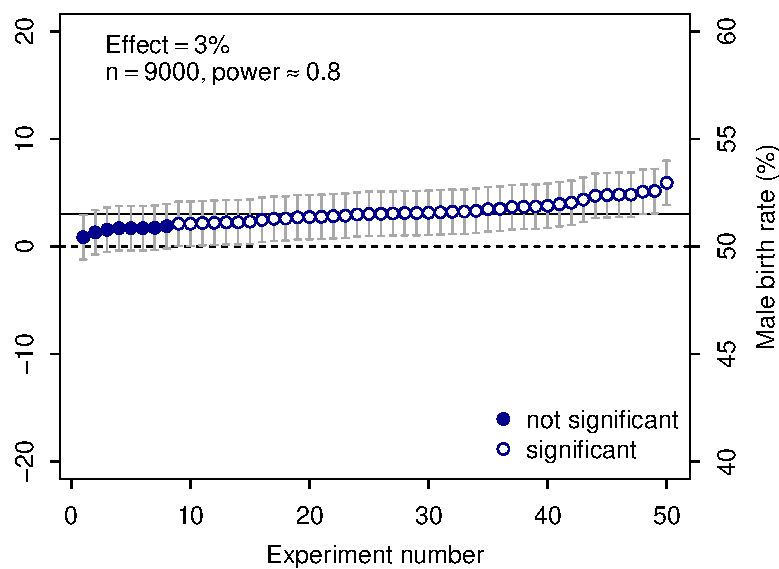
\includegraphics[width=7.9cm]{fig/birthdiff80}
\end{column}
\end{columns}

\vspace{2ex}

``If power is low \dots every possible outcome under repeated sampling will
be misleading: there will be a high proportion of inconclusive null results,
and any significant effects will be due to mis-estimations of the true
effect'' \citep[][p.~1317]{VasishthGelman21}

\end{frame}

% Why is high power so important for a study? Or conversely, why is low power
% so bad? A manifestation of the adverse consequences of low power is the
% replication crisis in science \citep{Gelman16, OSC15Science, Ioannidis05}.
% Hardly will effects be found again if they resulted from underpowered
% studies. It was long understood that low power leads to many non-significant
% tests and thus to uninformative studies \citep{Cohen90}. What was less
% obvious, however, is that in those cases when the test actually is
% significant, it gets even worse. What may look like a lucky shot -- one has
% managed to reach significance against the odds, so seemingly, the effect
% must be really large -- is a statistical artifact. If an underpowered test
% is significant, the magnitude of the effect will be exaggerated, sometimes
% strongly \citep[type M error;][]{ButtonIoannidis13, GelmanCarlin14,
% VasishthGelman21}. This is so, because with low power only the bizarrely
% extreme effect estimates will make it across the significance threshold
% \citep[for example][]{GelmanCarlin14, Gelman20}. And, still worse, the
% probability of the effect estimate having the wrong sign becomes high
% \citep[type S error;][]{Gelman14}. This is why high power is a necessary
% condition for valid inference from statistical tests. Failing to meet this
% condition renders misleading results.


\begin{frame}{Exercise: First steps in simulation}

\begin{itemize}
\item Generate data from a binomial model using the \texttt{rbinom()} function
in R;\\
try out different values of\\[1ex]
-- $n$ (10, 500, 2000)\\
-- the parameter $\pi$ (0.5, 0.8, 0.44, 0.515)\\[1ex]
and see how this affects the output\\[1ex]

\item With these data, test different null hypotheses using
\texttt{binom.test()};\\
these may or may not coincide with the values of $\pi$ used for data
generation\\[1ex]

\item If you repeat data generation and testing, can you usually reject H$_0$?
\end{itemize}

\end{frame}


%%%%%%%%%%%%%%%%%%%%%%%%%%%%%%%%%%%%%%%%%%%%%%%%%%%%%%%%%%%%%%%%%%%%%%%%%%%%%
\section{Power analysis by simulation}
%%%%%%%%%%%%%%%%%%%%%%%%%%%%%%%%%%%%%%%%%%%%%%%%%%%%%%%%%%%%%%%%%%%%%%%%%%%%%

\begin{frame}{Power analysis by simulation}

Why simulation?\\[1ex]
\begin{itemize}
\item Simulation is at the heart of statistical inference

\item Inference: Compare the data with the output of a statistical model

\item If data look different from model output, reject model (or its
assumptions)

\item Simulation forces us to {\bf specify a data model} and to attach meaning
to its components

\item Model should not be totally unrealistic for those aspects of the world
we want to learn about
\end{itemize}

\end{frame}

% How does one assure that the power of an experiment is high enough? And,
% first of all, how does one calculate the power of a planned test? This guide
% addresses both questions by computer simulation. But why calculate power by
% self-made simulation rather than by readily available software? Simulation
% forces us to specify a data model and to attach meaning to its components.
% This in turn will facilitate drawing valid inferences from the statistical
% test. After all, it is the model and its implications that the test
% confronts with empirical observations. Understanding what exactly is
% rejected if the test becomes significant, will improve our conclusions.


\begin{frame}{Power simulation}

The steps in general\\[1ex]

\begin{colbox}
\begin{enumerate}
\item Specify the model including the effect of interest

\item Generate observations from the model

\item Test H$_0$

\item Repeat
\end{enumerate}
\end{colbox}

\vspace{2ex}

Power is estimated from the proportion of significant test results

\end{frame}

% Ad 2: Once the data-generating model is fully specified, it can be used to
% draw observations from it. In R, functions like \verb+rbinom()+ or
% \verb+rnorm()+ will accomplish this. The number of draws equals the planned
% sample size of the experiment. Care has to be taken that the random sampling
% from the model reflects the design of the study. If there are dependencies
% in the data, as there are with repeated measures, the model has to produce
% correlated observations (for an example, see \ref{sec:pairtwosamplet}).
% These correlations have to be pre-specified as well.
%
% Ad 3: With the model-generated observations at hand one performs a test of
% H$_0$. The test should be the same as that which will be used to analyze the
% actual data, or else the power of the interesting test will remain unknown.


\begin{frame}{Specify the model including the effect of interest}

(1) Choose statistical model according to its assumptions
\begin{itemize}
\item Binomial test $\to$ binomial distribution $\to$ \texttt{rbinom()}

\item t-test $\to$ normal distribution $\to$ \texttt{rnorm()}

\item \dots\\[1ex]
\end{itemize}

(2) Fix unknown quantities
\begin{itemize}
\item Standard deviations, correlations, \dots \\[1ex]

%\item Plausible values from the literature (beware of significance filter)
\end{itemize}

(3) Specify the effect of interest
\begin{itemize}
%\item \emph{Not} the true effect (else no need to run the study!)

\item \emph{Not} the effect one expects or hopes to find (size of effect is
unknown!)

\item \emph{Never} an effect size taken from another study (significance
filter!)

\item \emph{But} the biologically or clinically or psychologically ``relevant
effect one would regret missing'' \citep{Harrell20}
\end{itemize}

\end{frame}

% This is the most crucial step, and it consists of several parts. First,
% choose the statistical model. For a parametric test, its assumptions
% predefine the distribution from which observations are drawn. For example, a
% binomial or a $t$ test requires the data to be binomially or normally
% distributed. Second, fix unknown quantities. In normal models, this requires
% fixing one or more standard deviations. Plausible values can be taken from
% the literature about broadly similar studies. One caveat is that reported
% standard deviations often are underestimates because of outlier removal and
% because focusing on significance filters out high values. Third, specify the
% effect of interest. Importantly, this is not the true effect or the effect
% one expects or hopes to find. One just does not know ahead of the experiment
% how large the effect will be; else one would not run the experiment in the
% first place. Also, it should never be an effect size taken from another
% study. Because of the significance filter, reported effect sizes are
% inflated. Rather, it should be the biologically or clinically or
% psychologically ``relevant effect one would regret missing''
% \citep{Harrell20}.


\begin{frame}[fragile]{Power simulation and sample size}

The steps in pseudo code\\[1ex]

\begin{lstlisting}[style=numbers]
  Set sample size to n
  replicate
  {
    Draw sample from model with minimum relevant effect
    Test null hypothesis
  }
  Determine proportion of significant results
\end{lstlisting}

\vspace{2ex}

Sample size calculation\\[1ex]

\begin{itemize}
\item Sample size $n$, minimal relevant effect and $\alpha$ must be
predetermined

\item Adjust $n$ until desired power ($0.8$ or $0.95$) is reached

\item To be on the safe side, assume higher variation, less (or more)
correlation, and smaller interesting effects (what results can we expect, if
\dots)
\end{itemize}

\end{frame}

% How is this procedure used for sample size calculation? This is
% straightforward. One starts with an arbitrary sample size (number of draws)
% and calculates the resulting power. If power is too low, one increases the
% sample size. This continues until the desired power level is reached. The
% goal here is not to find a single seemingly exact number. There are just too
% many unknowns: The model never matches exactly the true data-generating
% process, the standard deviations and correlations used in the simulation are
% only approximate, and more likely than not will there be invalid
% observations that have to be excluded due to reasons difficult to
% anticipate. Thus, for a realistic study, one should allow for some leeway by
% assuming higher variation, less (or more) correlation, and possibly smaller
% interesting effects. Yet, power simulation sets the frame of reference for
% interpreting the results. The question it answers is: What if? What results
% can we expect from a statistical test if the specified set of assumptions
% about the data-generating process were true?


%%%%%%%%%%%%%%%%%%%%%%%%%%%%%%%%%%%%%%%%%%%%%%%%%%%%%%%%%%%%%%%%%%%%%%%%%%%%%
\section{Examples and exercises}
%%%%%%%%%%%%%%%%%%%%%%%%%%%%%%%%%%%%%%%%%%%%%%%%%%%%%%%%%%%%%%%%%%%%%%%%%%%%%


\begin{frame}{Power simulation examples}

Binomial test\\[1ex]

\begin{itemize}
\item Birth rates in the general population\\[1ex]

\begin{tabular}{cc}
  
\includegraphics[scale=.1]{fig/babyboy} & 
  
\includegraphics[scale=.1]{fig/babygirl}\\
  51.5\,\% & 48.5\,\%\\
\end{tabular}

\item[$\to$] corresponds to a male-female sex ratio of 106:100\\[2ex]
\end{itemize}

More examples\\[1ex]

\begin{itemize}
\item \citet{Wickelmaier22} includes power simulation examples and R code for
many classical statistical tests
\end{itemize}

\end{frame}


\begin{frame}[fragile]{Example: Birth rates}

\begin{itemize}
\item Fisher's principle states that the male-female sex ratio is about
1:1\\[1ex]

\item Plan a study and calculate the sample size necessary to\\
-- detect a deviation from Fisher's principle of 106:100\\
-- with about 80\% power\\[1ex]

\item Check your setup\\
-- Set the effect size to zero; what ``power'' estimate do you expect to
get?\\[2ex]
\end{itemize}

\begin{lstlisting}[style=numbers]
n <- ...                                  # adjust sample size
pval <- replicate(5000, {                 # replications of experiment
  x <- rbinom(1, size = n,                # data-generating model with
              prob = 106/(106 + 100))     #   minimum relevant effect
  binom.test(x, n = n, p = 1/2)$p.value   # p-value of test against H0
})
mean(pval < 0.05)                         # simulated power at alpha = 0.05
\end{lstlisting}

\end{frame}

\begin{frame}[fragile]{Example: Birth rates}
  {Fisher's principle: Testing against H$_0$: $\pi = 0.5$}
  \begin{center}
    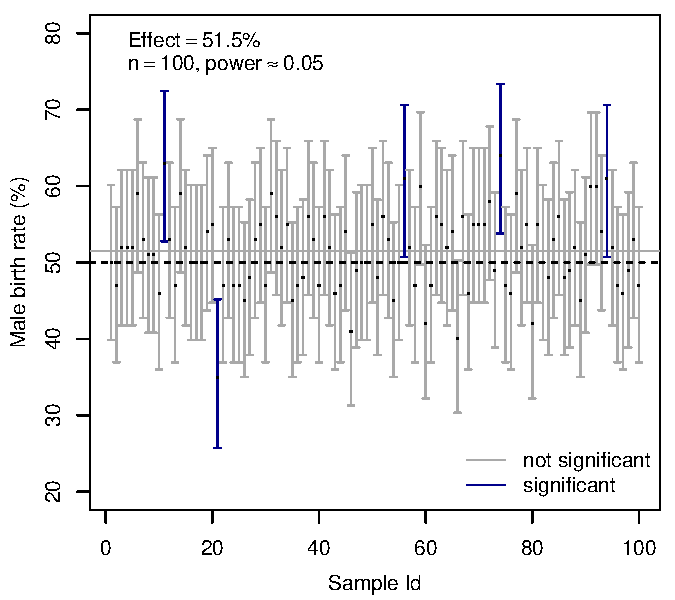
\includegraphics[scale=.7]{fig/ci_low}
  \end{center}
\end{frame}


\begin{frame}[fragile]{Example: Birth rates}
  {Fisher's principle: Testing against H$_0$: $\pi = 0.5$}
  \begin{center}
    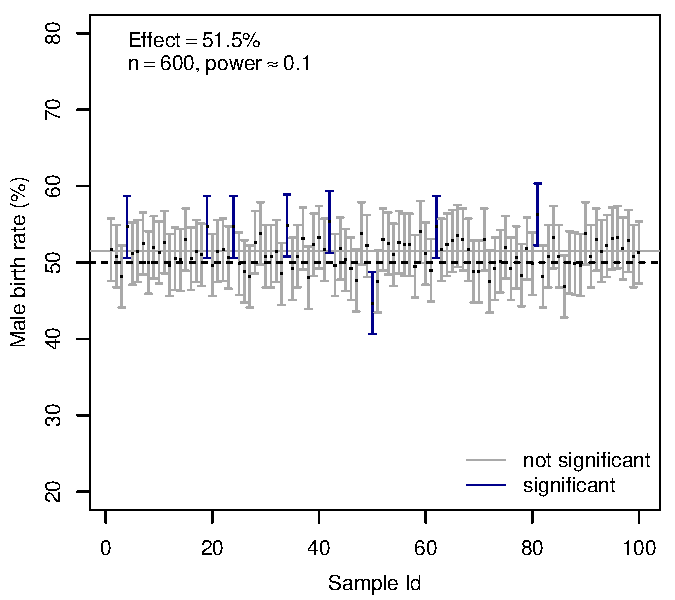
\includegraphics[scale=.7]{fig/ci_medium}
  \end{center}
\end{frame}


\begin{frame}[fragile]{Example: Birth rates}
  {Fisher's principle: Testing against H$_0$: $\pi = 0.5$}
  \begin{center}
    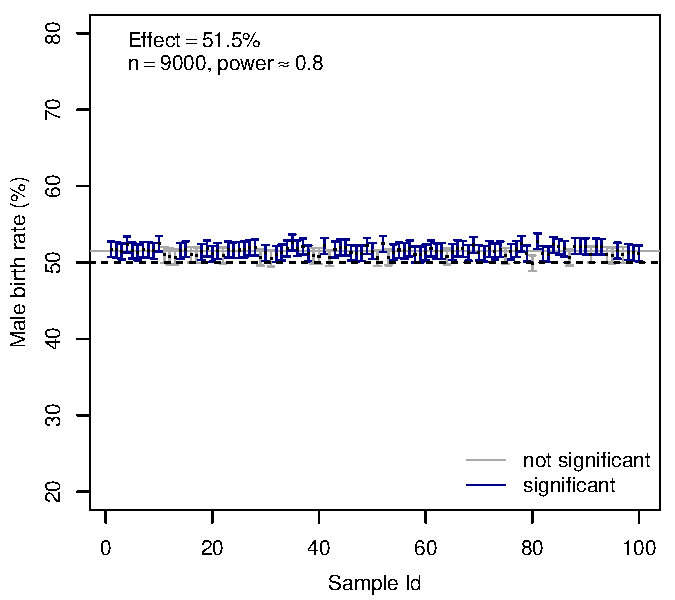
\includegraphics[scale=.7]{fig/ci_high}
  \end{center}
\end{frame}


% \begin{frame}{Exercise: Birth rates}
% 
% \begin{itemize}
% \item \citet{Kanazawa07} claims that beautiful parents have more
% daughters\\[1ex]
% 
% \item Plan a study and calculate the sample size necessary to\\
% -- detect a deviation from the global 106:100 male-female sex ratio\\
% -- with about 80\% power\\[1ex]
% 
% \item Wanted: Substance-matter knowledge\\
% -- What would be a minimum relevant deviation (effect)?\\
% -- Considering the literature on birth rates, what would be a realistic
% deviation?\\[1ex]
% 
% \item Some background\\
% -- \url{https://en.wikipedia.org/wiki/Human_sex_ratio}\\
% -- Literature cited there \citep[e.\,g.,][]{DavisGottlieb98,
% MathewsHamilton05}
% \end{itemize}
% 
% \end{frame}


\begin{frame}{Final thoughts}

~\hfill\begin{colbox}[10cm]
Statistical tests are no screening procedures\\[1ex]
-- Significance is not a substitute for relevance\\
-- Nonsignificance does not imply absence of effect
\end{colbox}\hfill~

\vspace{2ex}

\begin{itemize}
\item Often, data are rather uninformative and compatible with many models and
hypotheses\\[1ex]

\item At the same time, ``all models are wrong'' \citep{Box76}\\[1ex]

\item Making data-based decisions using statistical inference requires a
confirmatory setting where a-priori substantive knowledge goes into the power
analysis\\[1ex]

\item When relying on statistical tests outside such a setting, all we do is
descriptive statistics with p-values; this does more harm than good
\end{itemize}

\end{frame}


%%%%%%%%%%%%%%%%%%%%%%%%%%%%%%%%%%%%%%%%%%%%%%%%%%%%%%%%%%%%%%%%%%%%%%%%%%%%%

\appendix
\begin{frame}[allowframebreaks]{References}
\renewcommand{\bibfont}{\footnotesize}
\bibliographystyle{apacite}
\bibliography{../lit}
\end{frame}


\section{Extra slides}


\begin{frame}{P-value}

\begin{colbox}
The p-value is the probability of obtaining a test statistic that signals a
deviation from H$_0$ at least as extreme as that observed in the experiment,
given H$_0$ is true and its underlying model holds
\end{colbox}

\vspace{2ex}
\url{https://apps.mathpsy.uni-tuebingen.de/fw/pvalbinom/}

\end{frame}


\begin{frame}{On the role of power}

\begin{itemize}
\item \citet{VasishthGelman21}\\[1ex]

``the importance of power cannot be stressed enough. Power should be seen as
the ball in a ball game; it is only a very small part of the sport, because
there are many other important components. But the players would look pretty
foolish if they arrive to play on the playing field without the ball. Of
course, power is not the only thing to consider in an experiment; no amount of
power will help if the design is confounded or introduces a bias in some
way'' (p.~1333)
\end{itemize}

\end{frame}

\begin{frame}{Binomial test power simulation}

\begin{columns}
\begin{column}{7.9cm}
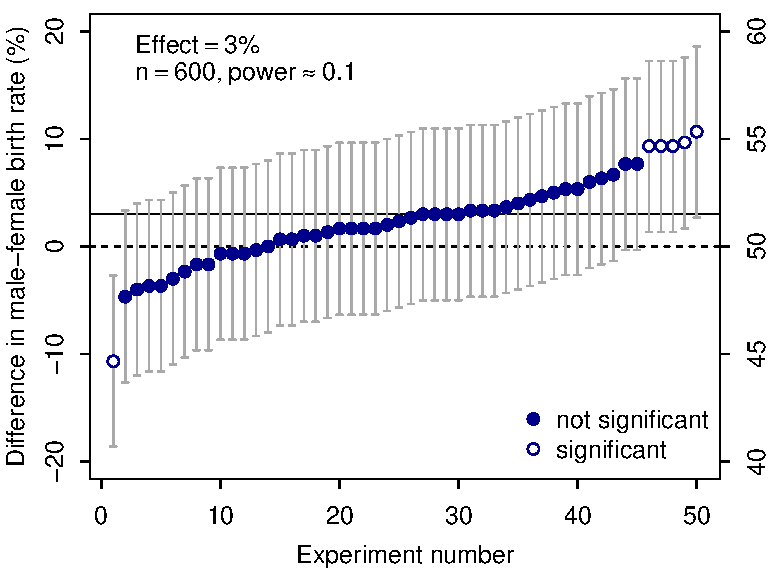
\includegraphics[width=7.9cm]{fig/birthdiff10}
\end{column}
%
\begin{column}{7.9cm}
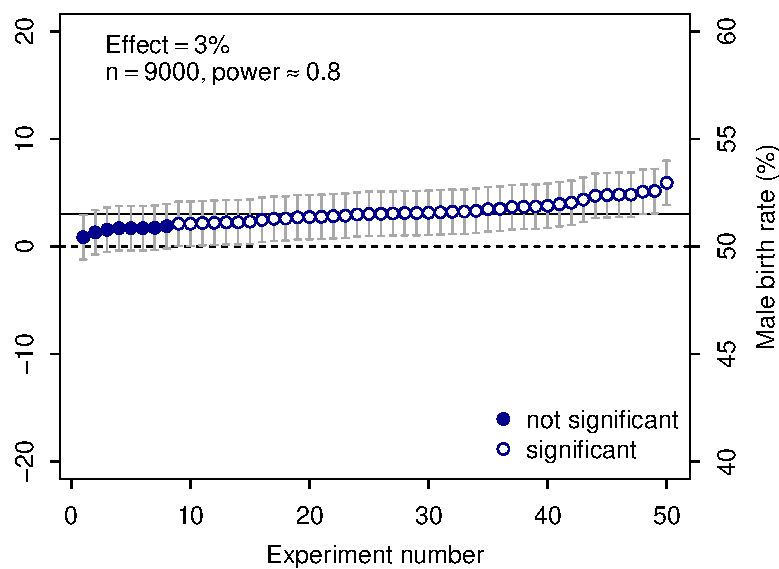
\includegraphics[width=7.9cm]{fig/birthdiff80}
\end{column}
\end{columns}

\vspace{2ex}

  \url{https://apps.mathpsy.uni-tuebingen.de/fw/birthrate/}

\end{frame}


\end{document}

